% Week 2 progress report; retains the Week 1 Springer LNCS template.
% Numerical sources: results/dpe/{five_seed_verification_20261112,
% ermstar_neural_two_seed_20261113,independent_methods_20261113}/.
% Qualitative screenshots copied unchanged from New folder/:
% 901975649_1153157754313840_5282200439323738894_n.png -> rotation_upright
% 904903694_2420140272139305_5586175427514070823_n.png -> rotation_beak_up
% 905261228_3327363100799798_3331977539064470536_n.png -> rotation_beak_down
% 906711406_29789600114061115_8522393143264929830_n.png -> rotation_half_turn
% 906058576_1619550210199352_3487361687074616956_n.png -> external_bird
\documentclass[runningheads]{llncs}
\IfFileExists{vietnam.sty}{\usepackage[utf8,nocaptions]{vietnam}}{\usepackage[utf8]{inputenc}}
\usepackage{graphicx}
\usepackage{booktabs}
\usepackage{float}
\setlength{\intextsep}{5pt}
\setlength{\tabcolsep}{5pt}
\usepackage{tabularx}
\usepackage{url}
\usepackage{tikz}
\usepackage[hidelinks]{hyperref}
\usetikzlibrary{arrows.meta,positioning,calc}
% Keep each method illustration with its caption and after its explanation.
\makeatletter
\newenvironment{methodfigure}{\par\medskip\noindent
  \begin{minipage}{\linewidth}\centering\def\@captype{figure}}
  {\end{minipage}\par\medskip}
\makeatother
\definecolor{dpeland}{HTML}{A65320}
\definecolor{dpewater}{HTML}{216B9B}
\definecolor{dpeink}{HTML}{263747}
\tikzset{
  dpe diagram/.style={font=\sffamily\scriptsize,text=dpeink,
    >=Stealth,line width=0.55pt},
  dpe box/.style={draw=dpeink!45,rounded corners=2pt,
    fill=dpeink!3,align=center,inner sep=4pt},
  dpe arrow/.style={->,draw=dpeink!75},
  dpe heading/.style={font=\sffamily\scriptsize\bfseries},
  dpe land/.style={circle,draw=dpeland,fill=dpeland!12,
    text=dpeland,minimum size=5mm,inner sep=1pt},
  dpe water/.style={rectangle,draw=dpewater,fill=dpewater!12,
    text=dpewater,minimum size=5mm,inner sep=1pt}
}
\begin{document}
\title{Background Shortcut Learning Mitigation for Waterbirds\texorpdfstring{\\}{: }
Week 2 Progress Report}
\titlerunning{Waterbirds: Week 2 Progress Report}
\author{Chau Tan Phat\inst{1,2} \and
Nguyen Dang Khang\inst{1,2} \and
Nguyen Phu Trong\inst{1,2} \and
Nguyen Dinh Minh Huy\inst{1,2}}
\authorrunning{C. T. Phat, N. D. Khang, N. P. Trong, N. D. M. Huy}
\institute{Faculty of Information Technology, University of Science, Ho Chi Minh City, Vietnam \and
Vietnam National University, Ho Chi Minh City, Vietnam\\
\email{ctphat2519@apcs.fitus.edu.vn, ndkhang2535@apcs.fitus.edu.vn}\\
\email{nptrong2530@apcs.fitus.edu.vn, ndmhuy2521@apcs.fitus.edu.vn}}
\maketitle

\raggedbottom
\section{Introduction}
The task is to classify a bird as a landbird or a waterbird. In Waterbirds, the training images usually show landbirds on land and waterbirds on water. A model may learn to look at the background instead of the bird. It can then fail when the background is misleading.

DPE (Diverse Prototypical Ensembles) uses 15 small classifiers, called \emph{heads}, to make one prediction. First, a ResNet-50 turns each image into a list of numbers describing it, called \emph{features}. We keep this network fixed. Each head learns from a different balanced subset and holds two \emph{prototypes}: one reference point for landbirds and one for waterbirds. These are learned vectors, not bird photos. Each head compares the image features with its two prototypes and gives a probability for each class. DPE averages the 15 answers (Fig.~\ref{fig:dpe-basic}).

\begin{methodfigure}
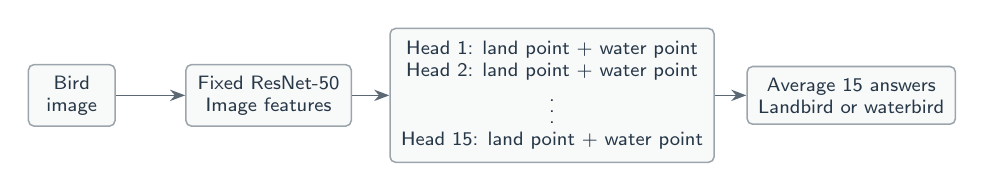
\begin{tikzpicture}[dpe diagram]
  \node[dpe box,minimum width=1.1cm] (image) at (0.5,0) {Bird\\image};
  \node[dpe box,minimum width=2.1cm] (net) at (3,0)
    {Fixed ResNet-50\\Image features};
  \node[dpe box,minimum width=3.2cm,minimum height=1.7cm] (heads) at (6.6,0)
    {Head 1: land point + water point\\Head 2: land point + water point\\$\vdots$\\Head 15: land point + water point};
  \node[dpe box,minimum width=2.1cm] (avg) at (10.4,0)
    {Average 15 answers\\Landbird or waterbird};
  \draw[dpe arrow] (image) -- (net);
  \draw[dpe arrow] (net) -- (heads);
  \draw[dpe arrow] (heads) -- (avg);
\end{tikzpicture}

\caption{Original DPE. Each head uses its own pair of reference points. All 15 answers count equally.}
\label{fig:dpe-basic}
\end{methodfigure}

\textbf{Evaluation.} We used 4,795 training, 1,199 validation, and 5,794 test images. We report \emph{worst-group accuracy} (WGA): the lowest accuracy among landbirds on land, landbirds on water, waterbirds on land, and waterbirds on water. Higher is better.

We averaged results over five standard ERM runs and two ERM$^*$ runs. ERM is ordinary training; ERM$^*$ trains longer with image augmentation. For learned combinations, 720 validation images train the heads and 479 fit the combination. We tried three such divisions, called Splits 0--2. Test labels were not used for these fits. The sections below return to our three Week 1 ideas and report what happened.

\newpage
\section{DPE Hypothesis Experiments}
\subsection{Changing Prototype Pairs}
\textbf{Obervation.} Each landbird prototype only competes with the waterbird prototype from its own head.

\textbf{Hypothesis.} Since heads learn from different images, swapping their prototype partners might give useful new comparisons without retraining.

\begin{methodfigure}
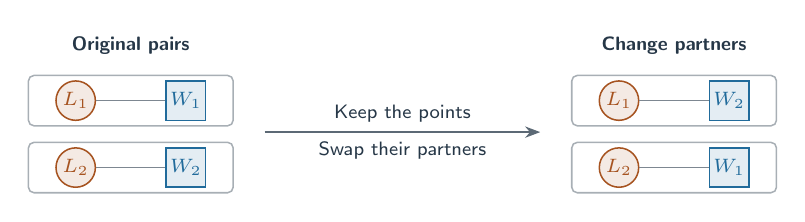
\begin{tikzpicture}[dpe diagram]
  \node[dpe heading] at (2,0.7) {Original pairs};
  \node[dpe heading] at (8.9,0.7) {Change partners};
  \foreach \i/\j/\y in {1/2/0,2/1/-0.85} {
    \draw[dpeink!40,rounded corners=2pt] (0.7,\y-.32) rectangle (3.3,\y+.32);
    \node[dpe land] (l\i) at (1.3,\y) {$L_\i$};
    \node[dpe water] (w\i) at (2.7,\y) {$W_\i$};
    \draw[dpeink!60] (l\i) -- (w\i);
    \draw[dpeink!40,rounded corners=2pt] (7.6,\y-.32) rectangle (10.2,\y+.32);
    \node[dpe land] (nl\i) at (8.2,\y) {$L_\i$};
    \node[dpe water] (nw\i) at (9.6,\y) {$W_\j$};
    \draw[dpeink!60] (nl\i) -- (nw\i);
  }
  \draw[dpe arrow] (3.7,-.4) -- (7.2,-.4)
    node[midway,above,align=center] {Keep the points}
    node[midway,below,align=center] {Swap their partners};
\end{tikzpicture}

\caption{Change partners, then average. $L$: landbird; $W$: waterbird. Numbers identify the original head. The points stay fixed.}
\label{fig:h1}
\end{methodfigure}

\textbf{Conclusion.} Shuffled pairs and all 225 possible pairs changed no final labels at the original scoring scales (Table~\ref{tab:pair-results}).

\begin{table}[!ht]
\centering
\caption{Our prototype-test WGA (\%): five normal-ERM runs, two ERM$^*$ runs. Ranges cover tested settings; global pooling shows its earlier highest mean. Dashes indicate untested settings, not zero accuracy.}
\label{tab:pair-results}
\small
\setlength{\tabcolsep}{5pt}
\begin{tabular}{@{}lrr@{}}
\toprule
Method & Normal ERM & ERM$^*$\\
\midrule
Uniform (our matched split baseline) & 89.23 & 93.42\\
Re-paired prototypes & 89.23 & ---\\
Larger prototype subsets (range) & 89.23--89.42 & 93.24--93.42\\
All 30 prototypes (earlier highest mean) & 89.30 & ---\\
\bottomrule
\end{tabular}
\end{table}

\subsection{Using More Prototypes per Head}
\textbf{Obervation.} Each head uses only two of 30 prototypes. One point may not cover a class's different appearances.

\textbf{Hypothesis.} Give each head several existing points per class. Compare the image with these points, add probabilities by class, then average the 15 heads.

\begin{methodfigure}

\begin{tikzpicture}[dpe diagram]
  \node[dpe heading] at (1.6,.8) {Original head};
  \node[dpe heading] at (5.6,.8) {More points per head};
  \draw[dpeink!40,rounded corners=2pt] (.4,-.38) rectangle (2.8,.38);
  \node[dpe land] at (1,0) {$L_1$};
  \node[dpe water] at (2.2,0) {$W_1$};
  \draw[dpe arrow] (3,0) -- (3.8,0);
  \draw[dpeink!40,rounded corners=2pt] (4,-.38) rectangle (7.2,.38);
  \node[dpe land] at (4.45,0) {$L_1$};
  \node[dpe land] at (5.2,0) {$L_2$};
  \node[dpe water] at (5.95,0) {$W_1$};
  \node[dpe water] at (6.7,0) {$W_2$};
  \node[dpe box,minimum width=2.8cm] (sum) at (9.7,0)
    {Compare with all four\\Add probabilities by class};
  \draw[dpe arrow] (7.2,0) -- (sum.west);
\end{tikzpicture}

\caption{Add points within each head. Subsets can differ. Using all 30 points with identical scoring makes every head's answer the same.}
\label{fig:h3}
\end{methodfigure}

\begin{table}[H]
\centering
\caption{Test WGA (\%), Split 0: five standard-ERM and two ERM$^*$ runs. Subsets use 2, 3, 5, or 15 pairs per head. The all-30 row is an earlier highest mean; a dash means untested.}
\label{tab:subset-results}
\small
\begin{tabular}{@{}lrr@{}}
\toprule
Prototypes per head & Standard ERM & ERM$^*$\\
\midrule
Original pair & 89.23 & 93.42\\
Larger subsets & 89.23--89.42 & 93.24--93.42\\
All 30 prototypes (earlier highest mean) & 89.30 & ---\\
\bottomrule
\end{tabular}
\end{table}

\subsection{Combining the Heads}
\textbf{Obervation.} DPE gives every head the same weight, even though the heads learned from different images.

\textbf{Hypothesis.} Some heads might rely more on backgrounds and make less useful predictions. Giving those heads less weight might improve the final answer. This was a possible explanation, not something we had already shown.

\begin{methodfigure}
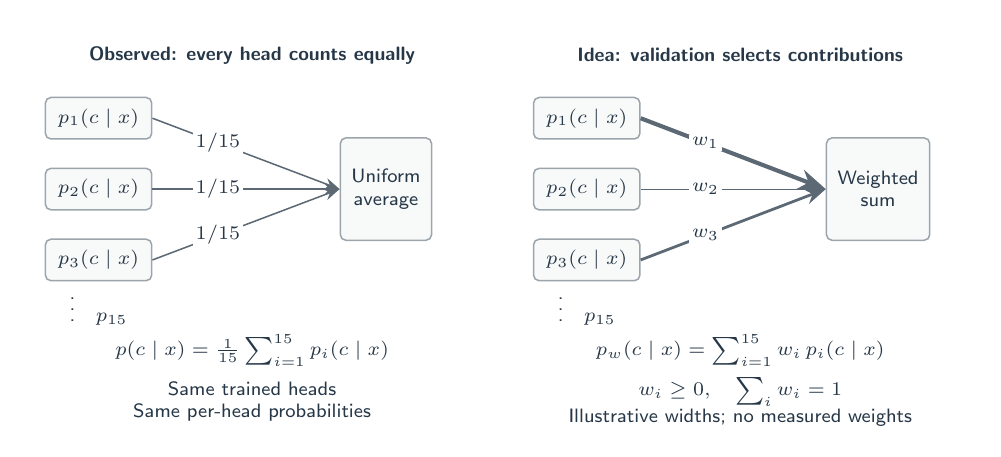
\begin{tikzpicture}[dpe diagram]
\path[use as bounding box] (-0.3,-4.65) rectangle (11.7,0.45);
\node[dpe heading] at (2.55,0.1) {Observed: every head counts equally};
\node[dpe heading] at (8.75,0.1) {Idea: validation selects contributions};
\foreach \i/\y in {1/-0.7,2/-1.6,3/-2.5} {
  \node[dpe box,minimum width=1.35cm] (a\i) at (0.6,\y) {$p_{\i}(c\mid x)$};
  \node[dpe box,minimum width=1.35cm] (b\i) at (6.8,\y) {$p_{\i}(c\mid x)$};
}
\node[dpe box,minimum height=1.3cm] (avg) at (4.25,-1.6) {Uniform\\average};
\foreach \i in {1,2,3} {
  \draw[dpe arrow] (a\i.east) -- (avg.west)
    node[pos=0.35,fill=white,inner sep=1pt] {$1/15$};
}
\node[dpe box,minimum height=1.3cm] (weighted) at (10.5,-1.6) {Weighted\\sum};
\draw[dpe arrow,line width=1.5pt] (b1.east) -- (weighted.west)
  node[pos=0.35,fill=white,inner sep=1pt] {$w_1$};
\draw[dpe arrow,line width=0.4pt] (b2.east) -- (weighted.west)
  node[pos=0.35,fill=white,inner sep=1pt] {$w_2$};
\draw[dpe arrow,line width=1pt] (b3.east) -- (weighted.west)
  node[pos=0.35,fill=white,inner sep=1pt] {$w_3$};
\node at (0.6,-3.05) {$\vdots\quad p_{15}$};
\node at (6.8,-3.05) {$\vdots\quad p_{15}$};
\node at (2.55,-3.65) {$p(c\mid x)=\frac{1}{15}\sum_{i=1}^{15}p_i(c\mid x)$};
\node at (8.75,-3.65) {$p_w(c\mid x)=\sum_{i=1}^{15}w_i\,p_i(c\mid x)$};
\node[align=center] at (8.75,-4.3) {$w_i\geq 0,\quad\sum_i w_i=1$\\Illustrative widths; no measured weights};
\node[align=center] at (2.55,-4.3) {Same trained heads\\Same per-head probabilities};
\end{tikzpicture}

\caption{The Week 1 idea: compare equal averaging with a weighted sum of the same head predictions. Here $p_i(c\mid x)$ is head $i$'s probability for class $c$ on image $x$. Arrow widths show example weights, not measured reliability.}
\label{fig:h2}
\end{methodfigure}

\textbf{What we tried.} Simple fixed weights did not help. We then learned a linear combination and a small network with 15 inputs and 8 hidden units. We also tried hiding 25\% of the inputs during training (\emph{dropout}). All heads are used at test time.

\begin{table}[H]
\centering
\caption{Test WGA (\%): our results and the original paper, labeled separately. Our means use five normal-ERM runs and two ERM$^*$ runs. The variants share our split-validation heads; full-validation reproduction uses all 1,199 validation images.}
\label{tab:combinations}
\small
\setlength{\tabcolsep}{5pt}
\begin{tabular}{@{}lrr@{}}
\toprule
How predictions are combined & Normal ERM & ERM$^*$\\
\midrule
Uniform (our split baseline) & 89.23 & 93.42\\
Linear combiner (our variant) & 89.56 & 94.00\\
Neural network (our variant) & 89.96 & 93.76\\
Dropout network (our variant) & 89.85 & 93.83\\
\midrule
DPE (our full-val. reproduction) & 89.60 & 94.08\\
\midrule
DPE (original paper) & 91.00 & 94.10\\
\bottomrule
\end{tabular}
\end{table}

The network raised standard-ERM WGA from 89.23\% to 89.96\% on Split 0, but the gains changed across splits and remain uncertain. On ERM$^*$, the learned combinations stayed below the 94.08\% result using all validation images. Saving images to fit the combination has a cost. We also have not shown that low-weight heads rely more on backgrounds.

We also tested three ways to change the final prediction without retraining the backbone:
\begin{itemize}
\item \textbf{Prototype weights:} learn how much each prototype contributes to the evidence for its class. The weights are learned separately for landbirds and waterbirds, using a loss that focuses on the worst group.
\item \textbf{Confidence adjustment:} keep the ordinary average of the heads and learn a scale and an offset for its prediction score. This can change confidence and the decision threshold, but does not use which heads disagree.
\item \textbf{Linear correction:} start with the same confidence adjustment, then add a learned weighted sum of each head's difference from the average. This lets the final answer respond to patterns of disagreement.
\end{itemize}
All three fits use validation data. Prototype weights use a 0.01 penalty; the two adjustments use 0.1. These penalties discourage large changes. The linear correction beat the simpler confidence adjustment on standard ERM, but lost to it on ERM$^*$.

\begin{table}[H]
\centering
% Fixed configurations: prototype-importance-shared-T0.05-maximum-l0.01;
% residual-affine-average-l0.1; residual-linear-average-l0.1.
\caption{Normal-ERM test WGA (\%; five runs). For each split, $\Delta$ is the change in percentage points from that split's matched uniform baseline. Positive is better. The full-validation reproduction and the paper are separate references; their data usage differs, so no matched-split change is reported for them.}
\label{tab:allocations}
\small
\setlength{\tabcolsep}{3pt}
\begin{tabular}{@{}lrrrrrr@{}}
\toprule
 & \multicolumn{2}{c}{Split 0} & \multicolumn{2}{c}{Split 1} & \multicolumn{2}{c}{Split 2}\\
Method & WGA & $\Delta$ & WGA & $\Delta$ & WGA & $\Delta$\\
\midrule
Uniform (matched baseline) & 89.23 & 0.00 & 90.12 & 0.00 & 89.70 & 0.00\\
Prototype weights & 90.55 & +1.32 & 90.10 & $-0.02$ & 88.51 & $-1.19$\\
Confidence adjustment & 89.76 & +0.53 & 90.30 & +0.18 & 89.90 & +0.20\\
Linear correction & 90.35 & +1.11 & 90.52 & +0.40 & 90.26 & +0.56\\
\midrule
DPE (our full-val. reproduction) & \multicolumn{6}{c}{89.60 (all validation images)}\\
DPE (original paper) & \multicolumn{6}{c}{91.00 (paper result)}\\
\bottomrule
\end{tabular}
\end{table}

\section{Predictions Viewer}
\subsection{Compare the Methods}
We built a browser viewer with 13 runs from DPE, AutoBackSwap, POTER, and ERM. It shows shared mistakes and disagreements. We can filter by bird species or bird/background group and inspect every method's answer for an image.

\begin{methodfigure}
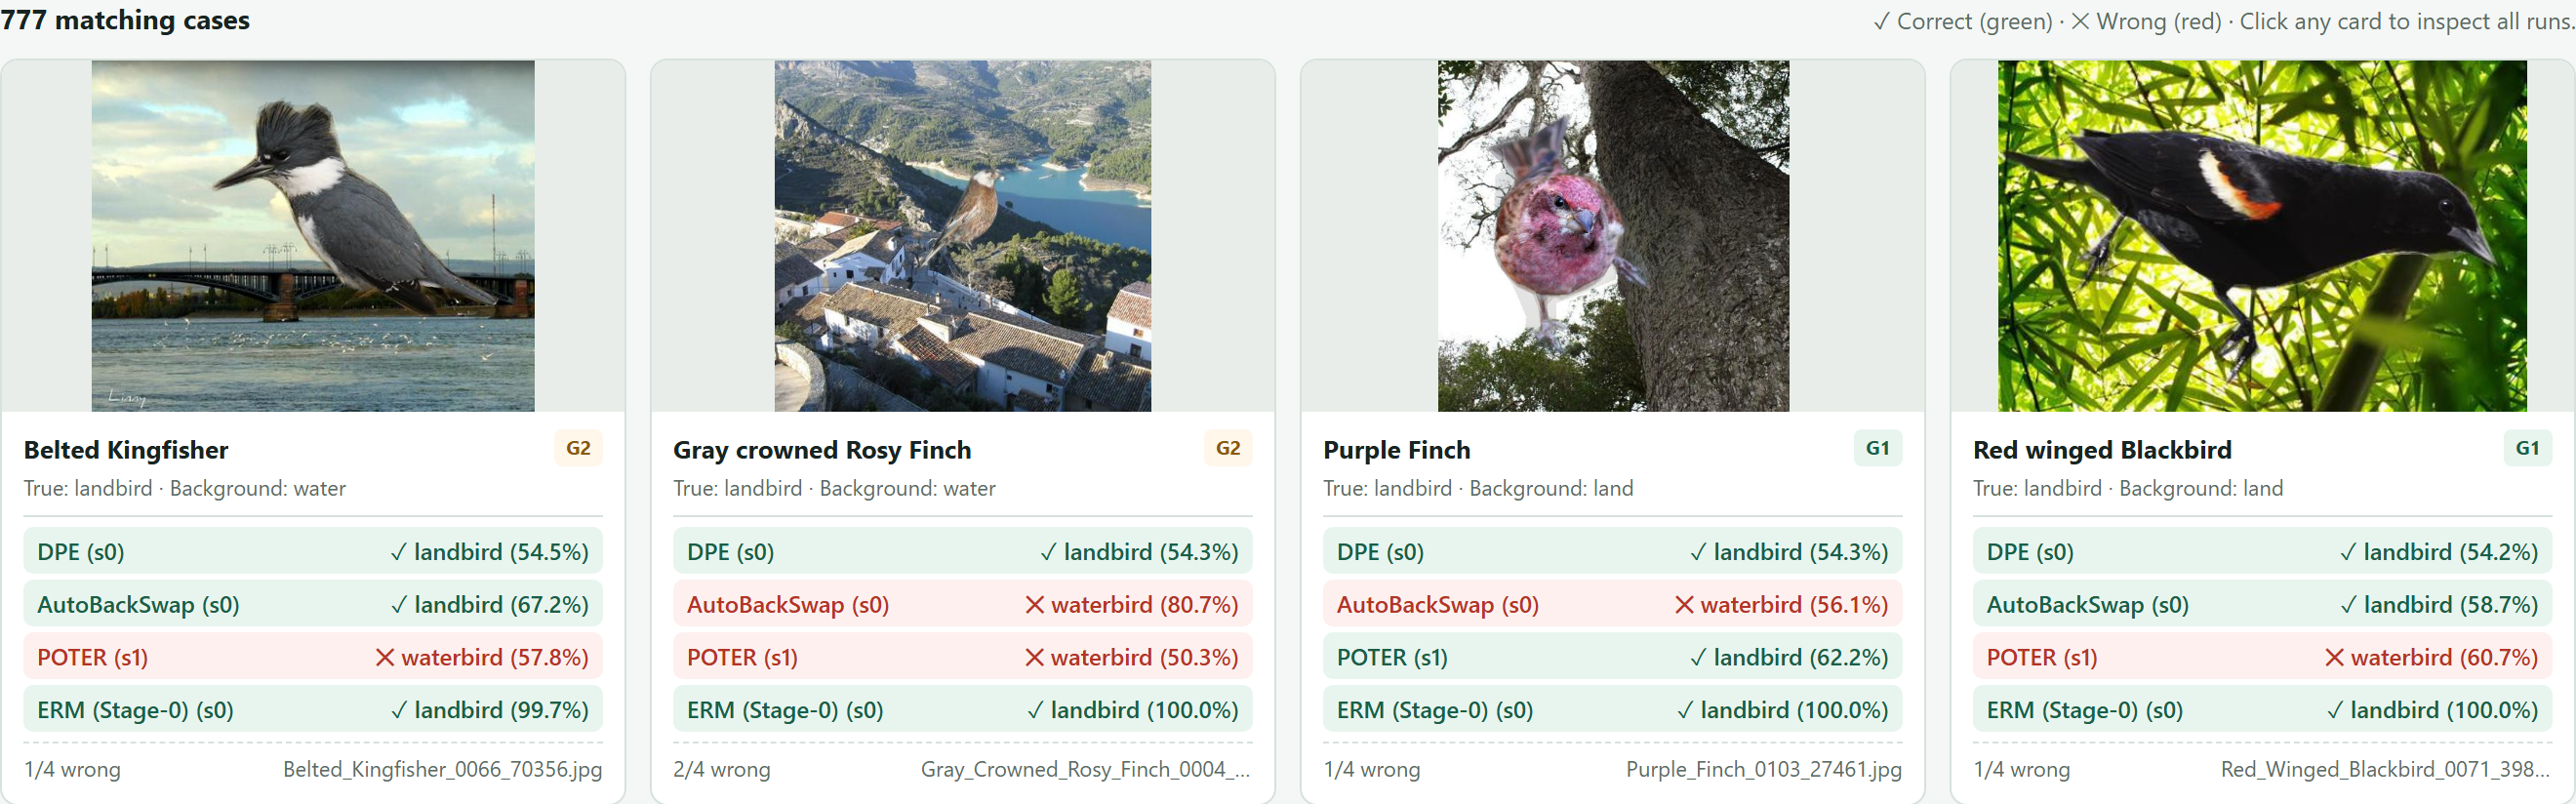
\includegraphics[width=\linewidth]{figures/week02_viewer.png}
\caption{The comparison viewer. Green agrees with the dataset label; red marks a mistake. In the second card, DPE and ERM are correct while AutoBackSwap and POTER are wrong.}
\label{fig:viewer}
\end{methodfigure}

\subsection{Rotation Test}
The supplied screenshots show a tool that runs inference with POTER. It displays the input image, the $224\times224$ crop seen by POTER, and the class probabilities. It also has a brush for editing the input. The screenshots below show predictions, not a controlled test of background edits.

For the same albatross on a land background, all four orientations were classified as waterbird. The probability changed from 90.79\% upright to 81.47\% with the beak upward, 72.81\% with the beak downward, and 75.02\% after a half-turn (Fig.~\ref{fig:rotation-check}). The class stayed the same, but one image is not enough to show rotation robustness.

\begin{methodfigure}
\begin{tabular}{@{}cccc@{}}
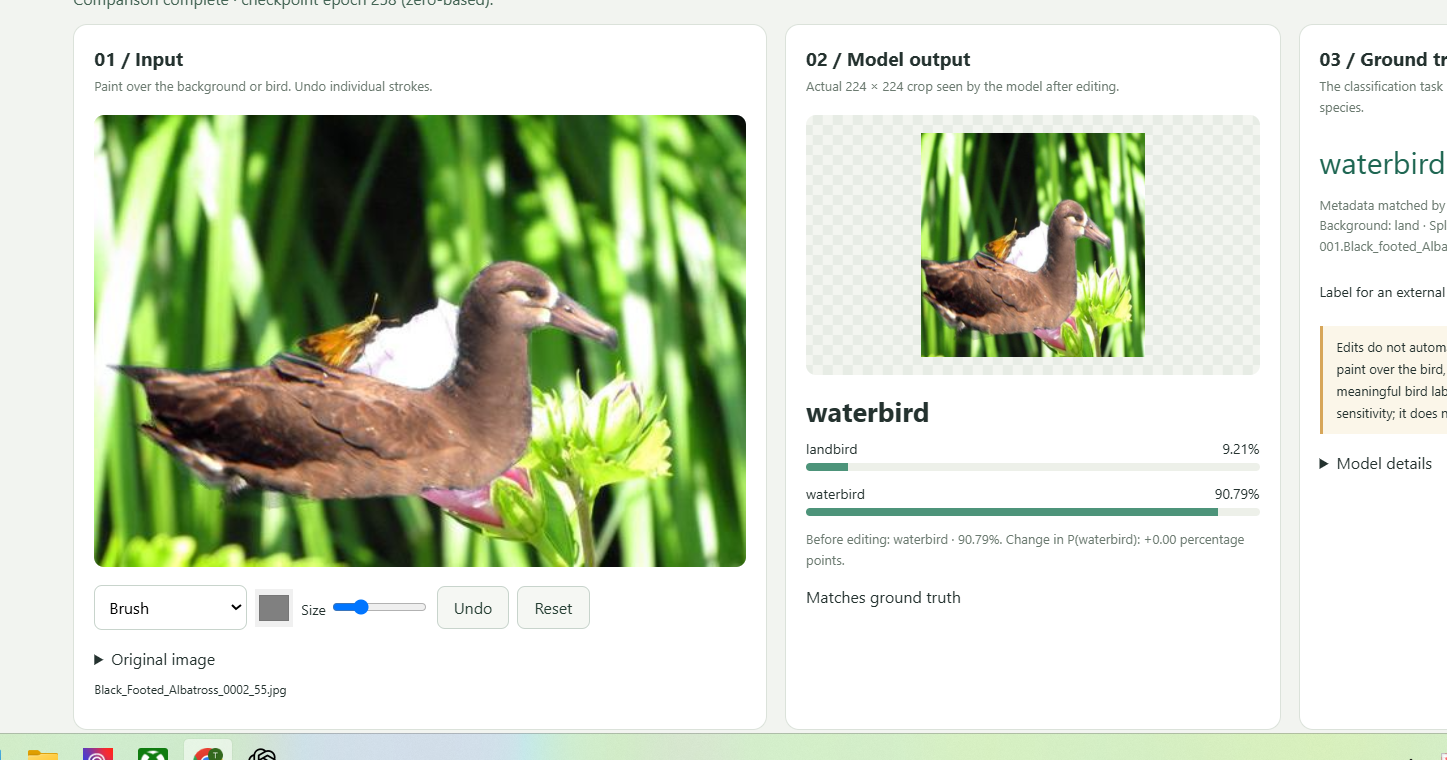
\includegraphics[width=0.225\linewidth,trim=800 240 180 115,clip]{figures/week02_rotation_upright.png} &
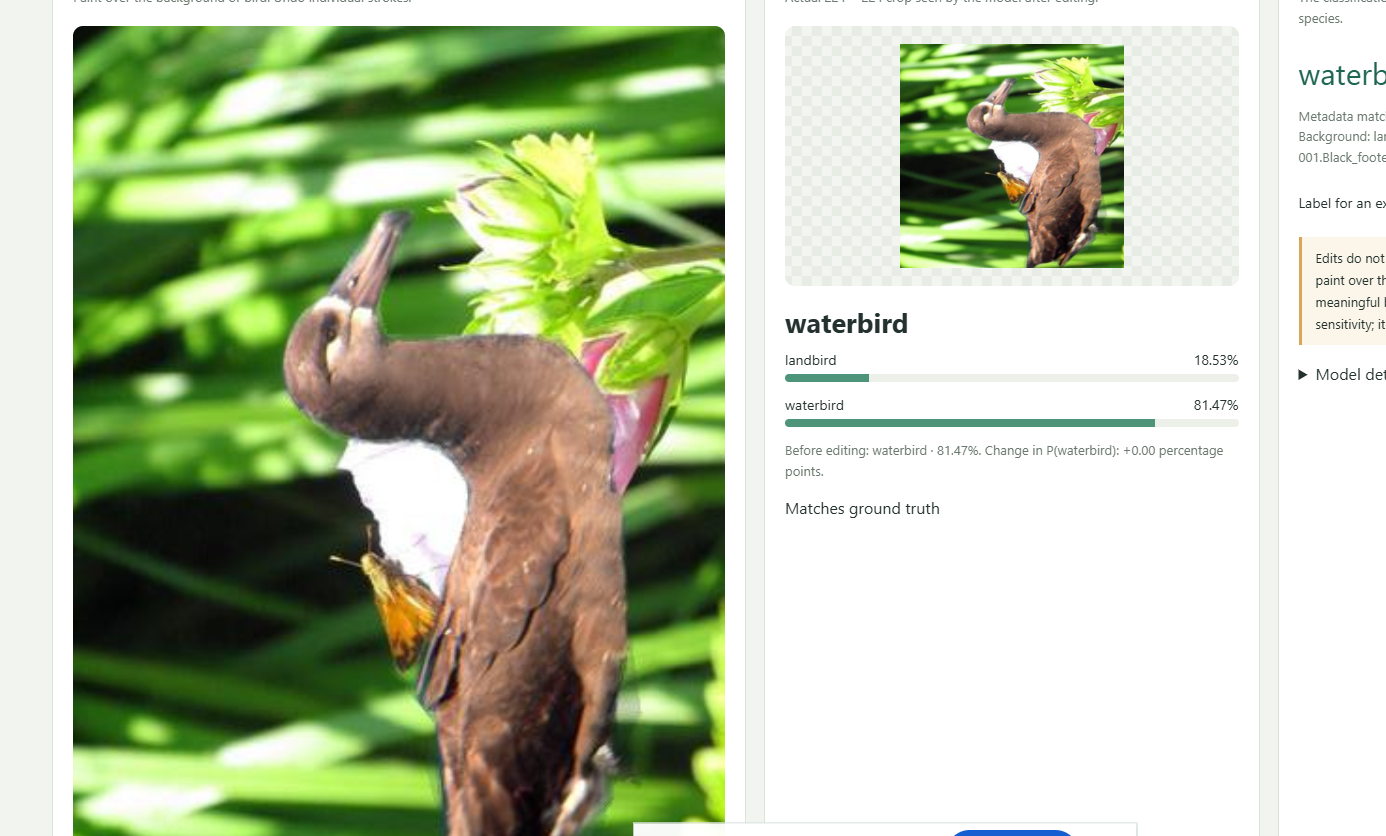
\includegraphics[width=0.225\linewidth,trim=780 405 140 25,clip]{figures/week02_rotation_beak_up.png} &
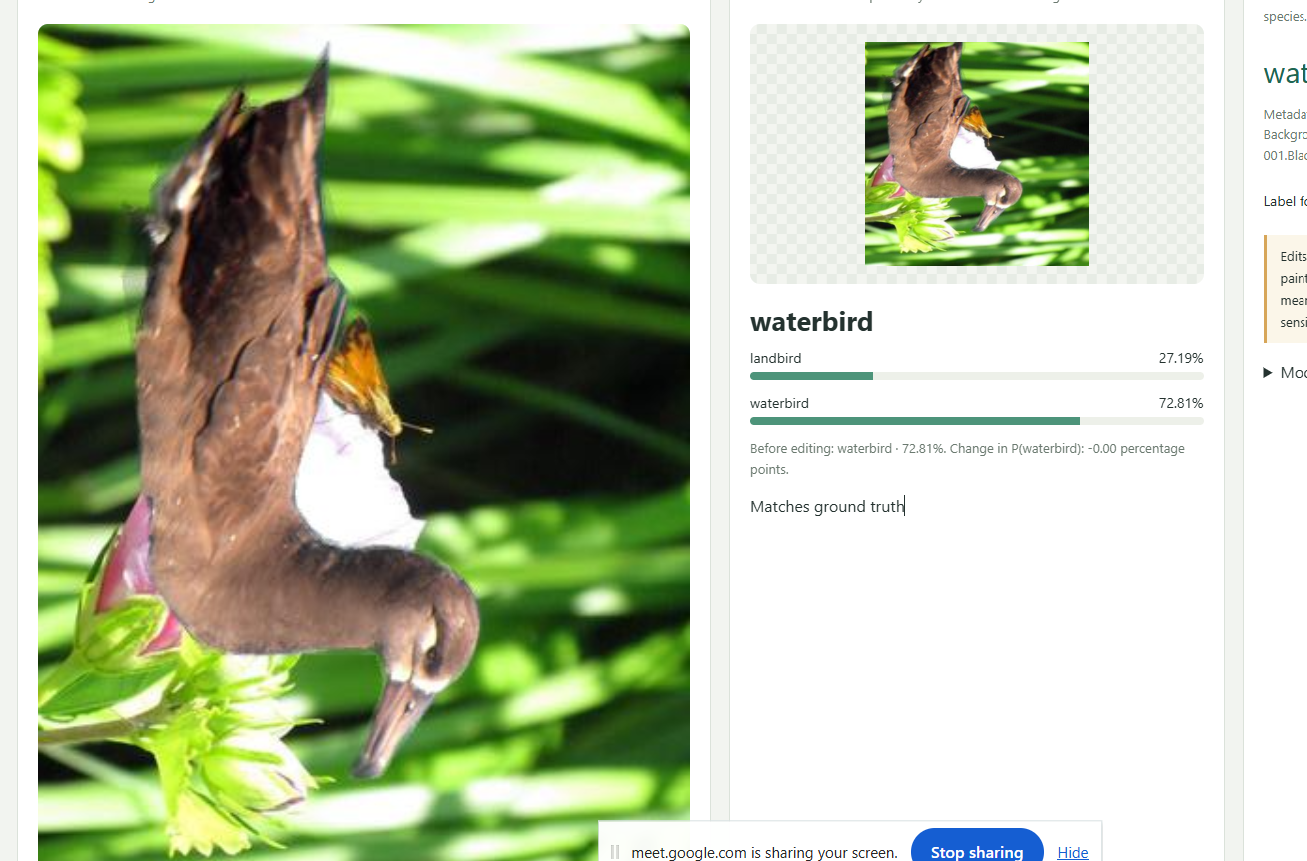
\includegraphics[width=0.225\linewidth,trim=745 430 100 23,clip]{figures/week02_rotation_beak_down.png} &
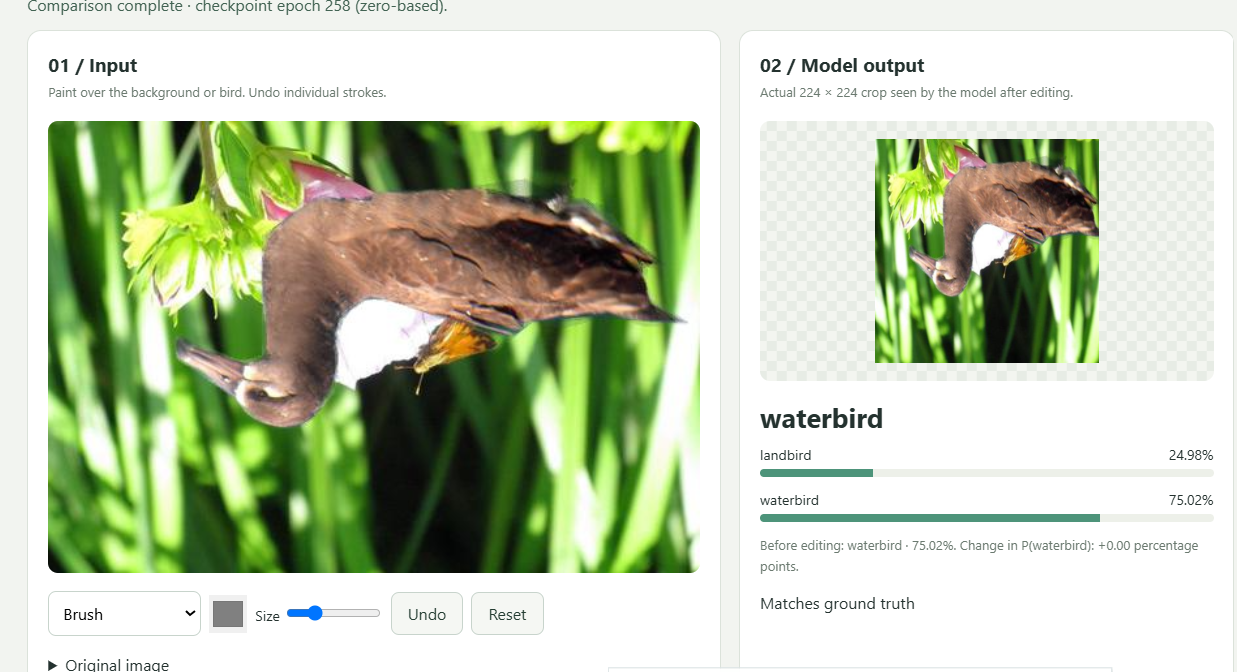
\includegraphics[width=0.225\linewidth,trim=755 145 20 120,clip]{figures/week02_rotation_half_turn.png}\\
\scriptsize Upright & \scriptsize Beak upward & \scriptsize Beak downward & \scriptsize Half-turn\\
\scriptsize 90.79\% & \scriptsize 81.47\% & \scriptsize 72.81\% & \scriptsize 75.02\%
\end{tabular}
\caption{POTER inference on four orientations of one albatross. Labels give the displayed waterbird probability. Panels are cropped from the supplied screenshots.}
\label{fig:rotation-check}
\end{methodfigure}

\subsection{Fused Image}
The images were first cropped into the correct square resolution. Then, for each pixel, the program takes a weighted average (in this case, 30\% bird01 and 70\% of bird06) of the RGB channel values.

POTER classified the fused bird image as landbird with probability 71.81\% (waterbird: 28.19\%), although the true label should be waterbird.

\begin{methodfigure}
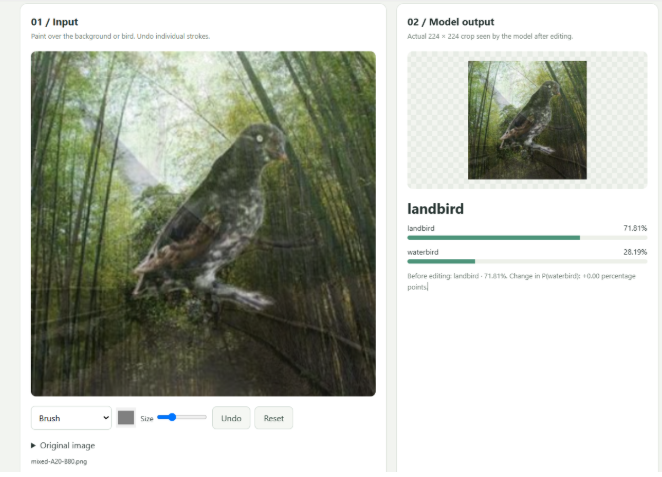
\includegraphics[width=0.6\linewidth]{figures/week02_external_bird.png}
\caption{POTER inference on the fused image. The left side shows the input; the right side shows the model crop and probabilities.}
\label{fig:external-check}
\end{methodfigure}

\textbf{Conclusion.} Changing prototype pairs did not change decisions. More prototypes per head gave little benefit. Learning how to combine heads gave some gains, but they depended on the validation split and the ERM setting. The test set has also been inspected before, so small gains need careful checking. Higher WGA alone does not prove that a model uses the background less.
\end{document}
